\documentclass[../main.tex]{subfiles}

\begin{document}

\section{Modeling with logarithmic functions}

Now it is turn to recall the logarithmic functions.
As before, first where are going to recap the definition of the logarithmic function and some of it's properties.
Then we are going to analyze some applications.

\begin{definition}{Logarithmic function}{log-fun-def}
    Consider a positive number $a$ with $a\neq1$.
    The logarithmic function with base $a$ is denoted as follows,
    \begin{gather*}
        f(x) = \log_a(x).
    \end{gather*}
    
    In a more mathematical/algebraic method to defined this function is by solving the problem of finding the inverse function of the exponential function.
    Hence, the most important property of the logarithmic functions is that,
    \begin{gather*}
        a^x\circ\log_a(x) = x.
    \end{gather*}
    
    Since it is the inverse function of the exponential function, the domain and range are swap from the exponential function, that is, $x\in\qty(0,\infty)$ and $f(x)\in\mathbb{R}$ or $f(x)\in\qty(-\infty,\infty)$, and has a vertical asymptote at $x=0$.

    \centering
    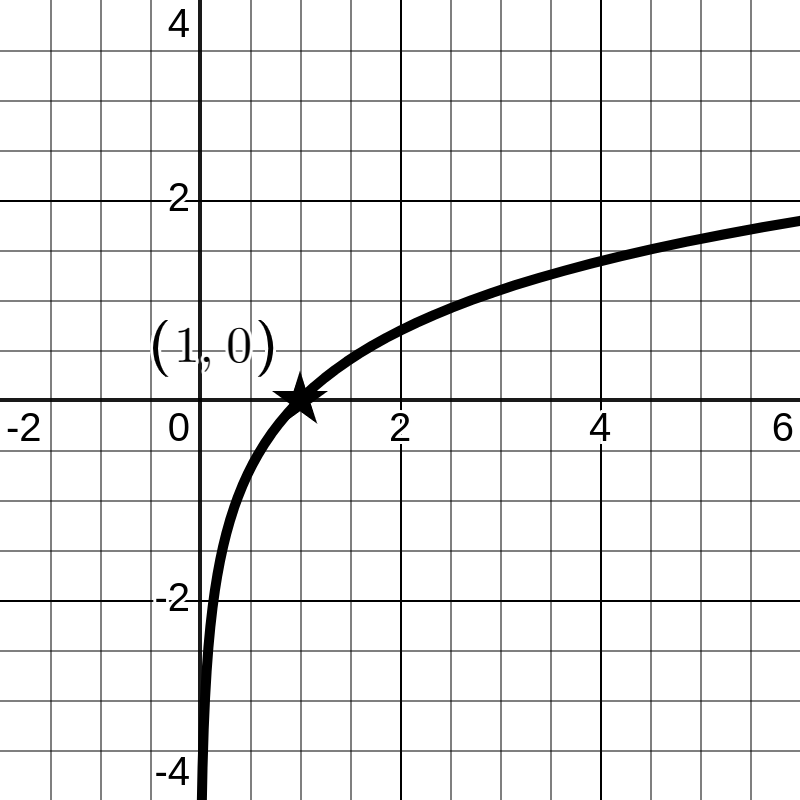
\includegraphics[width=0.4\textwidth]{imgs/log-graph.png}
\end{definition}

We can modify the function by adding the following parameters, $n_o,~r,~x_o$ and $f_o$,
\begin{gather*}
    f(x) = n_o \log_a\qty[r\qty(x-x_o)] + f_o.
\end{gather*}
The parameter $n_o$ controls how ``\textit{quickly}'' the function grows or decreases .
The parameter $r$ modifies the intersection with the $x$ axis.
The parameter $x_o$ moves the function to the left or right and the parameter $f_o$ shifts the horizontal asymptote up or down.
As a recommendation, try to plot in desmos an exponential function with those paramenters and play with them to see the transformations.

\subsection{Applications of the Logarithmic function}

As a difference with the exponential functions, the logarithmic functions, normally, doesn't have a direct application to describe a natural phenomena or process.
However, they are very usefull in data representation.
For example, if we want to compare the weight of different animals in a graph, got into a problem, because an ant weights \SI{0.0000003}{\kilo\gram}, an elephant \SI{4000}{\kilo\gram} and a whale \SI{170000}{\kilo\gram}.
So, when we try to graph those points (I suggest you to use desmos), the graphic is illegible.
However, if we plot them using a logarithmic scale we get the following values, \num{-5.5}, \num{3.6} and \num{5.2} for each animal.
Which help us to create a readable graph.

In science, the most common logarithmic scales are the pH scale, that measures the hydrogen ion concentration, the Richter scale, which measures the magnitude of an earthquake and the decibel scale, which measures the amount of power per area.
Now we are going to see an example of application,
\begin{example}{ph Scale and Hydrogen Ion Concentration}{lbl}
   The pH Scale is defined as follows,
   \begin{gather*}
        \mathrm{pH} = -\log\qty[\mathrm{H}^+].
   \end{gather*}
   where $\mathrm{H}^+$ represents the concentration of hydrogen ions measured n moles per liter.
   As general convention, solutions with a pH of 7 are defined as netural, those with $\mathrm{pH}<7$ are acidic, and those with $\mathrm{pH}>7$ are basic.
   (Consider that, when the pH increases by one unit, the hydrogen ions increases by a factor of 10.)

   Now, lets consider that the hydrogen ion concentration of a sample of human blod was measured to be $\mathrm{H}^+=\SI{3.16d-8}{\mole\per\liter}.$
   Find the $\mathrm{pH}$, and classify the blood as acidic or basic.

   We start by recalling the definition of the pH scale,
   \begin{gather*}
        \mathrm{pH} = -\log\qty[\mathrm{H}^+],
   \end{gather*}
   since, we know $\mathrm{H}^+ = \SI{3.16d-8}{\mole\per\liter}$,
    \begin{align*}
        \mathrm{pH} &= -\log\qty[\SI{3.16d-8}{\mole\per\liter}] \\
                    &= -\qty(-7.5) \\
                    &= 7.5.
   \end{align*}
   Hence, the blood sample is basic.

   
   As a final example, we are going to compute the concentration of hydrogen ions in the rain.
   Lets suppose that we measure the pH of the water from the rain and the intruments give us a lecture of 2.4, we can compute $\mathrm{H}^+$ as follows,
   \begin{align*}
        \mathrm{pH} &= -\log\qty[\mathrm{H}^+] \\
        2.4 &=  -\log\qty[\mathrm{H}^+] \\
        -2.4 &= \log\qty[\mathrm{H}^+] \\
        10^{-2.4} &=10^{\log\qty[\mathrm{H}^+]} \\
        10^{-2.4} &=\mathrm{H}^+ \\
        0.003981 &= \mathrm{H}^+. 
   \end{align*}
\end{example}

\subsection{Excersices}

\paragraph{a)} The hydrogen ion concentration of a sample of each substance is given.
Calculate the pH of the substance,
\begin{enumerate}
    \item Lemon juice: $\mathrm{H}^+=\num{5.0d-3}$
    \item Tomato juice: $\mathrm{H}^+=\num{3.2d-4}$
    \item Seawater: $\mathrm{H}^+=\num{5.0d-9}$
\end{enumerate}

\paragraph{b)} the pH reading of a sample of each substance is given.
Calculate the hydrogen concentration of the substance,
\begin{enumerate}
    \item Vinegar: pH = \num{3.0}
    \item Milk: pH = \num{6.5}
\end{enumerate}

\end{document}
